\chapter{General Purpose Graphics Processing Units}

\section{GPU architecture}
Graphics Processing Units (GPUs) were originally invented to accelerate computations revolving around 3D computer graphics. At the beginning of the 2000s, GPUs were discovered to offer enormous performance benefits over Central Processing Units (CPUs) when performing floating-point arithmetics. 

The hardware architecture of GPUs is fundamentally different from CPUs. CPUs are designed for sequential tasks, meaning that one instruction will be carried out after the other. Modern CPUs often consist of multiple \emph{cores}, from which the term \emph{multicore processor} arises \citep{hennessyComputerArchitectureQuantitative2012}. The cores in a multicore processor can all execute different instructions independently from each other. For example, one core might be occupied with the processing of a text document, while at the same time, another core might be busy rendering a video. Each core can fetch new instructions by itself and does not have to wait until the other cores have finished their current task. CPUs can be classified as Multiple Instruction Stream - Multiple Data Stream (MIMD) systems according to Flynn's taxonomy \citep{flynnVeryHighspeedComputing1966}. A modern high-end CPU can have in the order of tens of cores.

GPUs, on the other hand, are Single Instruction Stream - Multiple Data Stream (SIMD) systems. A SIMD system performs a single instruction on multiple data elements simultaneously. An example of such an operation is a vector addition; the instruction \emph{add} is performed on every pair of elements of the two vectors.

\begin{figure}[H]
    \centering
    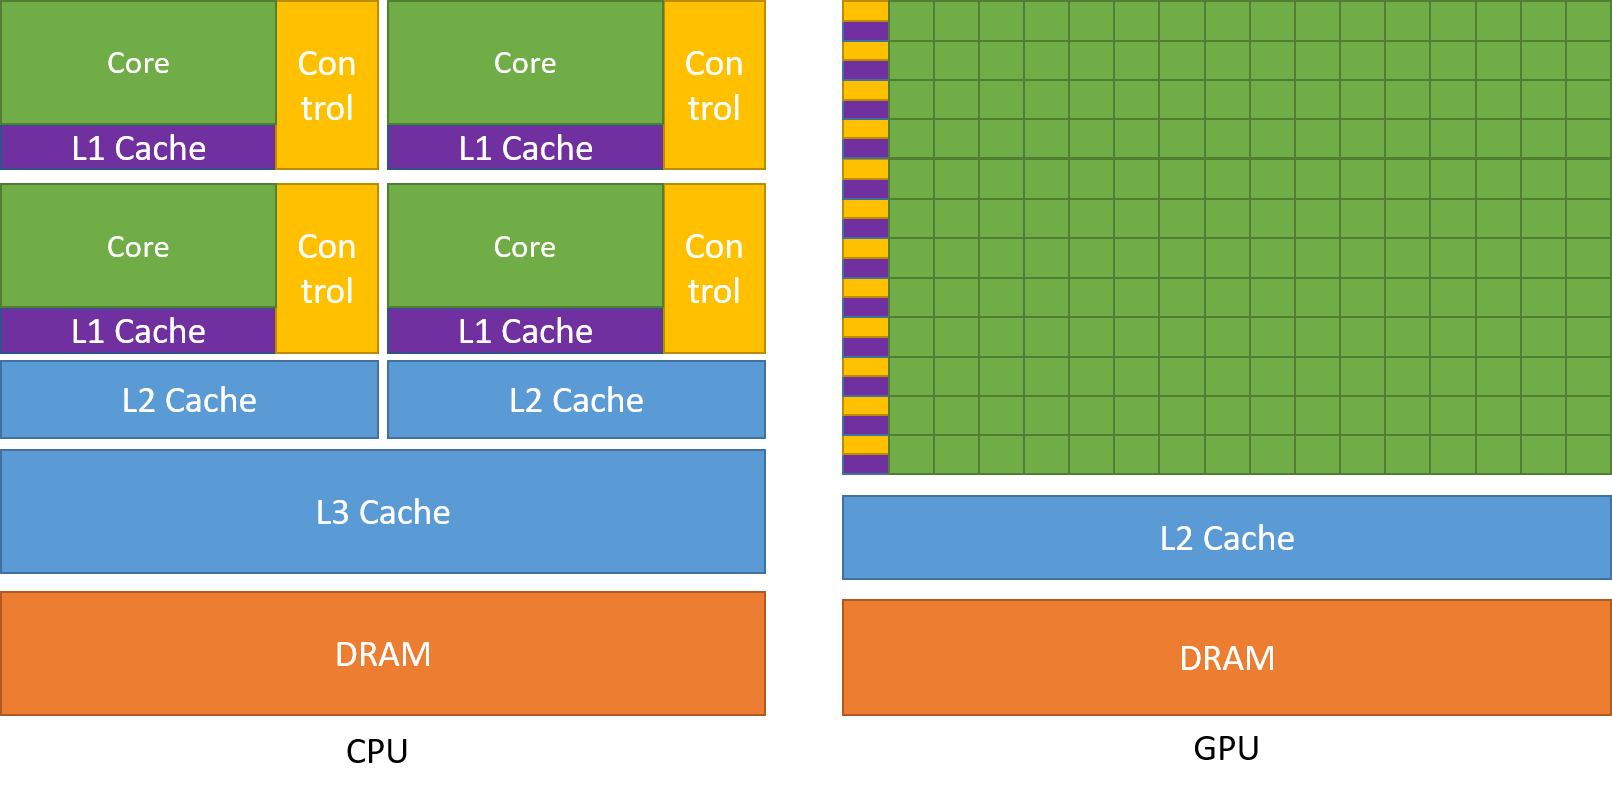
\includegraphics[width=0.7\textwidth]{../images/cpu-vs-gpu-diagram.png}
    \caption{Comparison between CPU and GPU architecture \citep{nvidiaCUDAProgrammingGuide2023}.}
    \label{fig:cpu-vs-gpu-diagram}
\end{figure}

\section{Programming GPUs} \label{sec:programming_gpus}
To exploit the capabilities of GPUs, specialized application programming interfaces (APIs) are available that provide access to the GPU hardware. Since GPUs were originally made for graphics processing, the first APIs were also tailored for that purpose. 

\textbf{Native kernel-based models} \\
Kernel-based methods involve writing function-like kernels that describe the computations that have to be done by a single thread of the GPU. At runtime, this kernel is then \emph{launched} across multiple threads, which all perform the kernel on a separate piece of data. \emph{Native} means that the API is designed for use with a specific family of GPUs. Perhaps the most well-known example of a native kernel-based model is NVIDIA's Compute Unified Device Architecture (CUDA). CUDA provides very fine-grained control over the GPU, thereby allowing for a great degree of optimization and consequently, the best performance. A drawback of CUDA is that it requires (partial) rewriting of existing code. If a CPU version of the program is required in addition to a GPU version, two separate versions of the code have to be maintained which is expensive and can introduce bugs. 

\textbf{Portable kernel-based models} \\
As opposed to native kernel-based models, portable kernel-based models are designed to work on hardware from a variety of vendors. A program still consists of kernels, but launching these kernels can be done with different backends of different vendors. The great benefit is that a program can run on different hardware without the need to rewrite the code, hence the name \emph{portable}. Upon compiling, the target hardware is selected, and the native code that can run on the selected hardware is generated. 

\textbf{Directive-based models} \\
A fundamentally different approach to GPU programming is the use of compiler directives. Compiler directives are instructions to the compiler to handle a section of code differently. These directives are placed near computationally expensive code - usually nested loops that iterate over large arrays - and the annotated code is converted to device code during compile time. Because directive-based methods do not require the writing of kernels, an application can be ported to GPUs in a relatively short amount of time. Two popular directive-based programming models are OpenACC and OpenMP.

\textbf{Standard language parallelism} \\
A more recent trend has been the implementation of parallel programming features directly in programming languages. An example is the Fortran \texttt{do concurrent} construct. Its usage is similar to directive-based models: parallelizing loops. With the right compiler, \texttt{do concurrent} loops can be executed on GPUs \citep{kedwardStateFortran2022}. A great benefit of standard language parallelism is that it is part of the syntax of the language, thus offering good usability for developers already familiar with the language. 

\textbf{Higher-level abstraction}
The last category of GPU programming models aims to abstract 

\section{GPUs in Supercomputers}

Number of accelerators in supercomputers over the years

Current trends (AI?)

\section{Related work}
\citet{niemeyerRecentProgressChallenges2014} have examined the status of GPU computing in the field of computational fluid dynamics (CFD). To demonstrate the potential benefits of using GPUs for CFD, two case studies were performed: a 2D Laplace equation, resembling the Poisson equation that is often found in CFD codes, and a lid-driven cavity flow. Four implementations were tested: single-core CPU, multi-core CPU with OpenMP, GPU with CUDA, and GPU with OpenACC. For mesh sizes up to $512^2$, the wall-clock time for the GPU implementations exceeded that of the multi-core CPU implementation. While the authors do not explicitly explore the possible causes of this behavior, it can be argued that the increase in wall-clock time is due to data transfer between the CPU and GPU. For larger mesh sizes, the GPU implementations outperformed the CPU implementations. Specifically, for the Laplace equation, the GPU solver showed a speedup of about 4.6, while for the lid-driven cavity flow, the speedup was about 2.8. Remarkably, \citet{niemeyerRecentProgressChallenges2014} showed that as the mesh size increases, the wall-clock time of the OpenACC implementation converged to that of the CUDA implementation.

DALES itself has been ported to GPUs before by \citet{schalkwijkHighPerformanceSimulationsTurbulent2012}. To this end, the original Fortran code of DALES was translated to C++, and calculations were moved to the GPU using CUDA, resulting in the GPU-resident Atmospheric Large-Eddy Simulation (GALES) model. \citet{schalkwijkHighPerformanceSimulationsTurbulent2012} found that GALES was able to reduce the wall-clock time per time step by a factor of 2 compared to DALES, although it should be noted that GALES uses single precision floating point numbers in most parts of the simulation, while DALES uses double precision. This is an important distinction to make, as GPUs are particularly well-optimized for single-precision floating point arithmetics. Since then, the company Whiffle has adopted GALES and further developed it into the GPU-Resident Atmospheric Simulation Platform (GRASP). GRASP is often used for very accurate simulations of windfarms \citep{verzijlberghAtmosphericFlowsLarge2021}.

\citet{costaFFTbasedFinitedifferenceSolver2018} has developed a tool for DNS of turbulent flows, called CaNS (Canonical Navier-Stokes solver). The dynamical core of CaNS is very similar to that of DALES: both use finite-difference discretization on a structured, staggered grid, an FFT-based solver for the pressure, and third-order Runge Kutta time integration. Unlike DALES, CaNS does not include a subgrid-scale model. Parallelization of CaNS is achieved by domain decomposition into pencils along two directions, with further shared-memory parallelization via OpenMP.
CaNS was later adapted for GPUs using CUDA Fortran \citep{costaGPUAccelerationCaNS2021}. CUDA Fortran provides a Fortran interface to the CUDA programming model and includes CUF Kernels. CUF Kernels are compiler directives that can be placed above loops to tell the compiler that the loop can be executed on the GPU. NVIDIA's cuFFT library was used to perform the FFT calculations on GPUs. Performance analysis was done on two systems: an NVIDIA DGX Station, a system comparable in size to a modern desktop PC and containing 4 Tesla V100 32 Gb GPUs, and an NVIDIA DGX-2, a standard 19-inch server chassis containing 16 Tesla V100 32 Gb GPUs. \citet{costaGPUAccelerationCaNS2021} found that for the same problem size, one would need about 6100 to 11200 CPU cores to match the wall-clock time per time step of the 16 Tesla V100s in the NVIDIA DGX-2. This is still a conservative estimate, as linear scaling was assumed for the CPU code, whereas in reality, performance often scales sublinearly for a given problem size due to overhead introduced by communication between processes. For reference, the first phase of the new TU Delft DelftBlue supercomputer has around 11,000 CPU cores, indicating that GPUs can offer a significant reduction in energy consumption.
